\documentclass{beamer}

\usepackage{tcolorbox}
\usepackage{graphicx}

%\beamerdefaultoverlayspecification{<+->}
\newcommand{\data}{\mathcal{D}}

\DeclareMathOperator*{\argmin}{arg\,min}

\newcommand\Item[1][]{%
	\ifx\relax#1\relax  \item \else \item[#1] \fi
	\abovedisplayskip=0pt\abovedisplayshortskip=0pt~\vspace*{-\baselineskip}}


\usetheme{metropolis}           % Use metropolis theme


\title{Linear Regression}
\date{\today}
\author{Nipun Batra and the teaching staff}
\institute{IIT Gandhinagar}
\begin{document}
  \maketitle
  
  
  
% \section{Linear Regression}

\begin{frame}{Linear Regression}
\begin{itemize}
	
	
	\item<+-> O/P is continuous in nature.
	\item<+-> Examples of linear systems:
	\begin{itemize}
		\item<+-> $F=ma$
		\item<+-> $v=u+at$
	\end{itemize}
	
\end{itemize}
\end{frame}

\begin{frame}{Task at hand}
\begin{itemize}

\item TASK: Predict Weight = F(Height)
\end{itemize}
\begin{center}
    

\begin{tabular}{ |c|c|c|c| } 
\hline
 Height & Weight \\
\hline
3 & 29 \\ 
4 & 35 \\ 
5 & 39\\
2 & 20\\
6 & 41\\
\hline
\hline
7 & ?\\
8 & ?\\
1 &? \\
\hline
\end{tabular}

\end{center}
The first part of the dataset are the training points. The latter ones are testing points.	

\end{frame}



\begin{frame}{Scatter Plot}
\begin{center}
        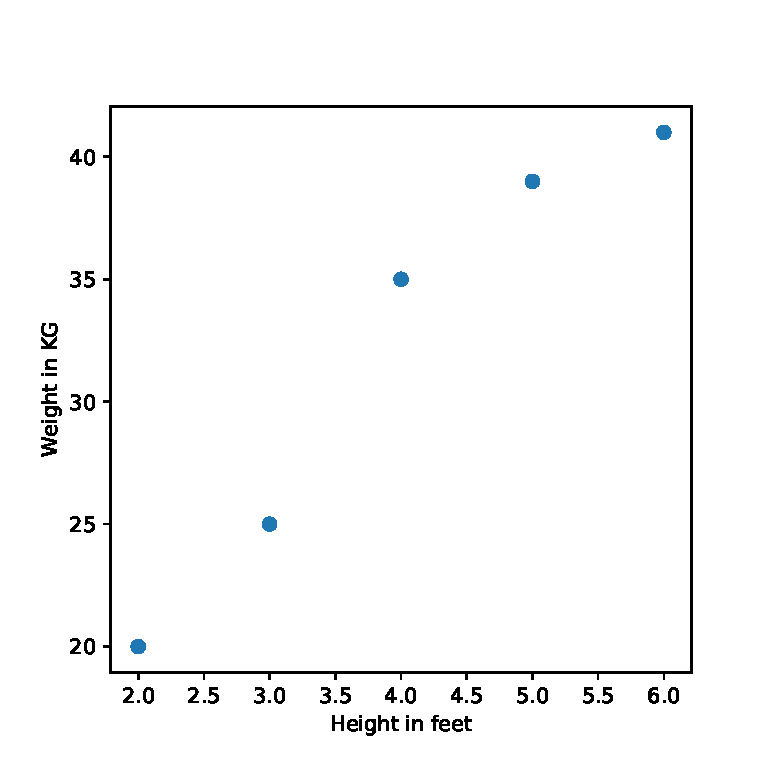
\includegraphics[totalheight=6cm]{linear-reg/height-weight-scatterplot.eps}
        

        
\end{center}


\end{frame}

\begin{frame}{Matrix representation of the expression}
\begin{center}
\begin{tcolorbox}
$weight_{i}$ $\approx$
$\theta_{0}$+$\theta_{1}$*$height_{i}$
\end{tcolorbox}
\end{center}

\begin{itemize}
\item $weight_{1}$ $\approx$
$\theta_{0}$+$\theta_{1}$*$height_{1}$

\item $weight_{2}$ $\approx$
$\theta_{0}$+$\theta_{1}$*$height_{2}$


\item $weight_{N}$ $\approx$
$\theta_{0}$+$\theta_{1}$*$height_{N}$

\end{itemize}
\end{frame}

\begin{frame}{Matrix representation of the expression}



\[\begin{bmatrix}
    weight_{1}   \\
    weight_{2}   \\
    \dots \\
    weight_{N}
\end{bmatrix}
= \begin{bmatrix}
    1& height_{1}   \\
    1& height_{2}   \\
    \dots & \dots  \\
    1& height_{N}   \\
\end{bmatrix}
\begin{bmatrix}
    \theta_{0} \\
    \theta_{1}
\end{bmatrix}\]
\[W=X\theta \]


W(N \times 1); X(N\times 2); \theta(2 \times 1);


\begin{itemize}
    \item<+-> $\theta_{0}$ - Bias Term
    \item<+-> $\theta_{1}$ - Intercept Term
\end{itemize}
\end{frame}



\begin{frame}{Extension to multiple dimensions}

In the previous example y = F(x), where x is one-dimensional.\\
Examples in multiple dimensions.\\
One example is to predict the water demand of the IITGN campus

\small{
\begin{center}
    \begin{tcolorbox}
        Demand = F(\# occupants, Temperature)
    \end{tcolorbox}
\end{center}

\begin{center}
    \begin{tcolorbox}
        Demand = Base Demand + $K_{1}$ * \# occupants + $K_{2}$ * Temperature
    \end{tcolorbox}
\end{center}
}

\end{frame}

\begin{frame}{Intuition}
    We hope to: 
    \begin{itemize}
        \item Learn $F$: $Demand$ = $F(\# occupants, Temperature)$
        \item From training dataset
        \item To predict the condition for the testing set
    \end{itemize}
\end{frame}


\begin{frame}{Linear Relationship}
    We have 
    \begin{itemize}
        \item $demand_{i} = \theta_{0} + \theta_{1} X_{i,1} + \theta_{2} X_{i,2} + \dots$
        \item $demand_{i} = x_{i}^{T} \theta$
    \end{itemize}
    Both of the above are the same.\\
    \textbf{Notice the transpose in the second equation! This is because $x_{i}$ is a column vector} 
\end{frame}


\begin{frame}{Linear Relationship}
    So, $y_{i}$ = $\hat{y_{i}}$ + $\epsilon_{i}$, where
    \begin{itemize}
        \item $y_{i}$ denotes the ground truth for $i^{th}$ sample
        \item $\hat{y_{i}}$ denotes the prediction for $i^{th}$ sample, where $\hat{y_{i}}$ = $x_{i}^{T} \theta$
        \item $\epsilon_{i}$ denotes the error for $i^{th}$ sample
    \end{itemize}
\end{frame}



\begin{frame}{We can expect the following}
    \begin{itemize}
        \item<+-> Demand increases, if \# occupants increases, then $K_{1}$ is likely to be positive
        
        \item<+-> Demand increases, if temperature increases, then $K_{2}$ is likely to be positive
        
        \item<+-> Base demand is independent of the temperature and the \# occupants.
        
    \end{itemize}
\end{frame}



\begin{frame}{Generalized Linear Regression Format}


    \[\begin{bmatrix}
        y_{1}\\
        y_{2} \\
        \vdots \\
        y_{N}
    \end{bmatrix}
    =     \begin{bmatrix}
        1 & x_{11} & x_{12} & \dots & x_{1m}\\
        1 & x_{21} & x_{22} & \dots & x_{2m}\\
        \vdots & \vdots & \vdots & \dots & \vdots\\
        1 & x_{N1} & x_{N2} & \dots & x_{Nm}\\
        % y_{2} \\
        % \vdots \\
        % y_{N}
    \end{bmatrix}
    \begin{bmatrix}
        \theta_{0}\\
        \theta_{1}\\
        \vdots \\
        \theta_{m}\\
    \end{bmatrix}
   \]
   
%   \begin{center}
%       \textbf{Y}: N\times1; \textbf{X}: N\times(M+1); $\mathbf{\theta}$: (M+1)\times1 
%   \end{center}
   
   \begin{tcolorbox}
   \begin{center}
       
   

   $ Y \approx X\theta$
   \end{center}
   \end{tcolorbox}
   
   \begin{itemize}
       \item<+-> We have N knows, (or N equations)
       \item<+-> M unknowns (or M parameters/ variables)
   \end{itemize}
   
\end{frame}


\begin{frame}{Relationships between feature and target variables}
    
    There are different $\theta_{0}$ $\&$ $\theta_{1}$. Each of them can represents a relationship.\\
    \vspace{0.5em}
    Given multiples values of $\theta_{0}$ $\&$ $\theta_{1}$ how to choose which is the  best?
    
\end{frame}
\begin{frame}{Error terms}
\begin{itemize}
    \item $\theta_{0}, \theta_{1}$: The parameters of the linear regressions
    \item $\epsilon_{i}$: Variable residual per example 
\end{itemize}


\begin{equation*}
    \epsilon_{i} = y_{i} - \hat{y}_{i}
\end{equation*}
\begin{equation*}
    \epsilon_{i} = y_{i} - (\theta_{0} + x_{i}\times\theta_{1})
\end{equation*}
\end{frame}



\begin{frame}{Good fit}

\begin{itemize}
    \item<+-> $|\epsilon_{1}|$, $|\epsilon_{2}|$, $|\epsilon_{3}|$, ... should be small.
    \item<+-> 
${\text{minimize }} \epsilon_{1}^2 + \epsilon_{2}^2 + \dots + \epsilon_{N}^2$ - $L_{2}$ Norm
    \item<+-> 
${\text{minimize }} |\epsilon_{1}| + |\epsilon_{1}| + \dots + |\epsilon_{1}|$ - $L_{1}$ Norm
\end{itemize}
\end{frame}



\begin{frame}{Normal Equation}
    
    
    \begin{tcolorbox}
       $ Y = X\theta + \epsilon$
    \end{tcolorbox}
    
    To Learn: $\theta$ \\
    Objective: ${\text{minimize }} \epsilon_{1}^2 + \epsilon_{2}^2 + \dots + \epsilon_{N}^2$  
\end{frame}

\begin{frame}{Normal Equation}
    
\begin{equation*}
 \epsilon = 
\begin{bmatrix}
    \epsilon_{1} \\
    \epsilon_{1} \\
    \vdots \\
    \epsilon_{N} \\
\end{bmatrix}
\end{equation*}
\\
\begin{center}
    Minimize $\epsilon^{T}\epsilon$    
\end{center}
\end{frame}

\begin{frame}{Derivation of Normal Equation}
\begin{align}
\label{eqn*:eqlabel}
\begin{split}
   \epsilon &= y - X\theta \\
\epsilon^{T} &= (y-X\theta)^{T} = y^{T} - \theta^{T}X^{T}\\
\epsilon^{T}\epsilon &= (y^{T} - \theta^{T}X^{T})(y - X\theta)\\
&=y^{T}y - \theta^{T}X^{T}y - y^{T}X\theta+\theta^{T}X^{T}X\theta\\
&=y^{T}y - 2y^{T}X\theta+\theta^{T}X^{T}X\theta
\end{split}
\end{align}

This is what we wish to minimize
\end{frame}

\begin{frame}{Minimizing the objective function}
    
    
    \begin{equation}
        \frac{\partial \epsilon^{T} \epsilon}{\partial \theta} = 0    
    \end{equation}
    
    
    
    \begin{itemize}
        \item $
    \cfrac{\partial }{\partial \theta} y^{T}y= 0
    $
    \item $
    \cfrac{\partial }{\partial \theta}(-2y^{T}X\theta ) = (-2y^{T}X)^{T} = -2X^{T}y
    $
    \item $ \cfrac{\partial}{\partial\theta} (\theta^{T}X^{T}X\theta) = 2X^{T}X\theta$
    \end{itemize}
    
    Substitute the values in the top equation
    
\end{frame}

\begin{frame}{Normal Equation derivation}
$$
    0 = -2X^{T}y + 2X^{T}X\theta
$$

$$
    X^{T}y  = X^{T}X\theta
$$

\begin{tcolorbox}
\begin{center}
    

        $\theta = (X^{T}X)^{-1}X^{T}$
\end{center}
\end{tcolorbox}

\end{frame}

\begin{frame}{Worked out example}
    \begin{center}
 \begin{tabular}{||c c||} 
 \hline
 x  & y \\ [0.5ex] 
 \hline\hline
 0 & 0 \\
 1 & 1 \\
 2 & 2 \\
 3 & 3 \\
 \hline
\end{tabular}
\end{center}

Given the data above, find $\theta_{0}$ and $\theta_{1}$.

\end{frame}


\begin{frame}{Scatter Plot}
\begin{center}
            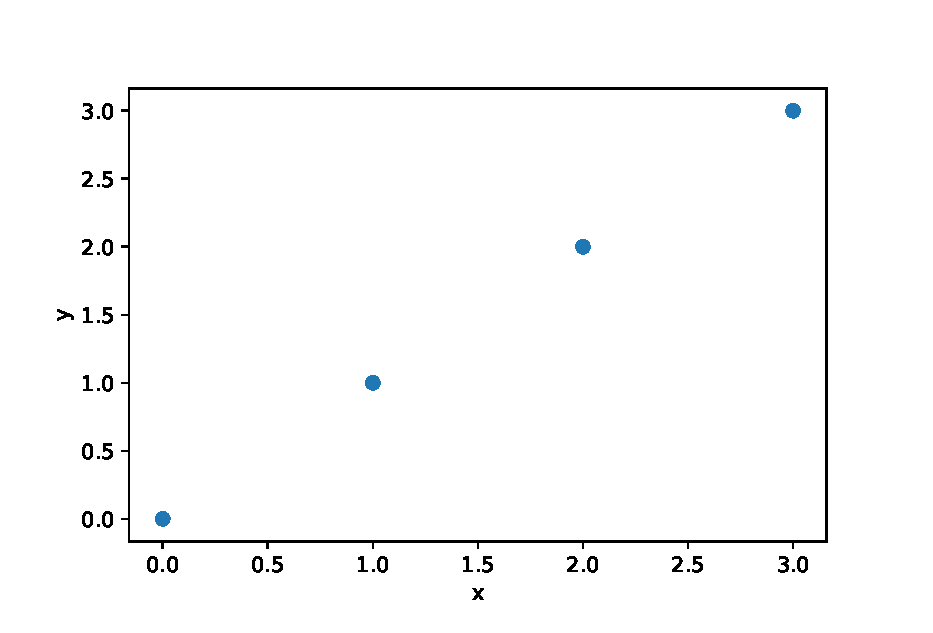
\includegraphics[totalheight=6cm]{linear-reg/scatterplot-2.eps}
\end{center}
    
\end{frame}


\begin{frame}{Worked out example}
\begin{align}
    \begin{split}
        X &= \begin{bmatrix}
            1 & 0\\
            1 & 1\\
            1 & 2\\
            1 & 3
        \end{bmatrix}\\
        X^{T} &= \begin{bmatrix}
            1&1&1&1\\
            1&2&3&4
        \end{bmatrix}\\
        X^{T}X &= \begin{bmatrix}
            4 &6\\6&14
        \end{bmatrix}
    \end{split}
\end{align}
Given the data above, find $\theta_{0}$ and $\theta_{1}$.
\end{frame}


\begin{frame}{Worked out example}
    \begin{align}
        \begin{split}
            (X^{T}X)^{-1} &= \frac{1}{20} \begin{bmatrix}
                14 & -6\\
                -6& 4
            \end{bmatrix}\\
            X^{T}y &= \begin{bmatrix}
                6\\
                14
            \end{bmatrix}
        \end{split}
    \end{align}
\end{frame}


\begin{frame}{Worked out example}
    \begin{align}
        \begin{split}
            \theta &= (X^{T}X)^{-1}(X^{T}y)\\
            \begin{bmatrix}
        \theta_{0}\\
        \theta_{1}
    \end{bmatrix} &= 
    \begin{bmatrix}
        0\\
        1
    \end{bmatrix} 
        \end{split}
    \end{align}
\end{frame}


\begin{frame}{Effect of outlier}

    \begin{center}
 \begin{tabular}{||c c||} 
 \hline
 x  & y \\ [0.5ex] 
 \hline\hline
 0 & 0 \\
 1 & 1 \\
 2 & 2 \\
 3 & 3 \\
 4 & 0 \\
 \hline
\end{tabular}
\end{center}

Compute the $\theta_{0}$ and $\theta_{1}$.
\end{frame}
\begin{frame}{Scatter Plot}
    
    \begin{center}
        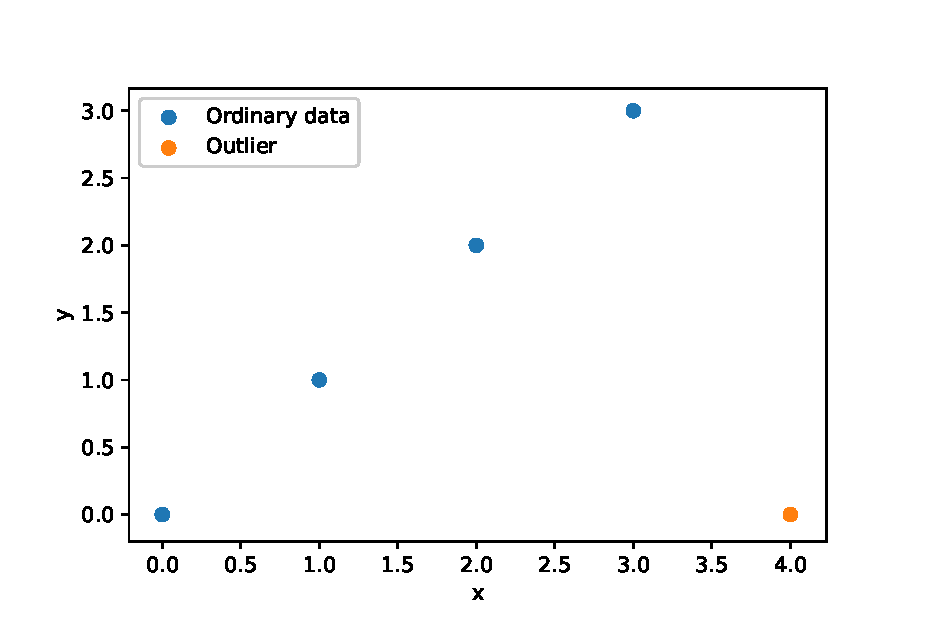
\includegraphics[totalheight=6cm]{linear-reg/scatterplot-3.eps}
\end{center}

\end{frame}


\begin{frame}{Effect of outlier}
    
    \begin{center}
        \begin{bmatrix}
        $\theta_{0}$\\
        $\theta_{1}$
        
    \end{bmatrix}
     = 
     \begin{bmatrix}
        2\\
        -\frac{1}{5}
    \end{bmatrix}
    \end{center}
    
\end{frame}

\begin{frame}{Model fit}
    
       
    \begin{center}
        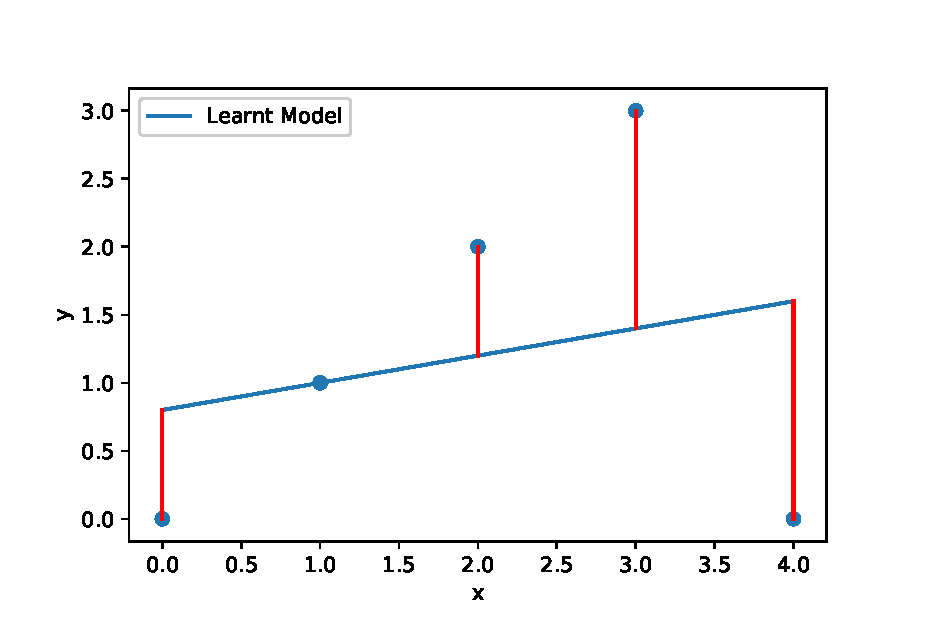
\includegraphics[totalheight=6cm]{linear-reg/linear-fit.eps}
    \end{center}



\end{frame}
% \begin{frame}{Frame Title}
    
%     \begin{align}
        
%         \begin{split}
%             \theta &= \frac{1}{20}\begin{bmatrix}
%                 14 & -6\\
%                 -6 & 4
%             \end{bmatrix}
%             \begin{bmatrix}
%                 6\\
%                 14
%             \end{bmatrix}\\
%             &= \frac{1}{20} \begin{bmatrix}
%                 0 \\
%                 20
%             \end{bmatrix}\\
            
%             % \begin{bmatrix}
%             %     \theta_{0}\\
%             %     \theta_{1}
%             % \end{bmatrix}
%             %  = 
%             %  \begin{bmatrix}
%             %      0 \\
%             %      1
%             %  \end{bmatrix}
%         \end{split}
%     \end{align}
%     $$
% \end{frame}

\begin{frame}{Quick Question}
    
    $$
    y = X\theta;
    $$
    
    Can we do
    $$theta = X^{-1}y$$
    
    Why? or why not?
    
\end{frame}


\begin{frame}{Quick Question}

    X may not be a square matrix. So, $X^{-1}$ may not exist.
    
    Rectangular matrices have a left inverse and a right inverse.
\end{frame}



\begin{frame}{Relation between \#instances and \# Variables}
    
    If N$<$ M, then it is an under-determined system\\
    Example: N=2; M=3\\
 
   $$ \begin{bmatrix}
        30 \\
        40 
    \end{bmatrix}
     = \begin{bmatrix}
         1 & 6& 30\\
         1 & 5& 20
     \end{bmatrix}    \begin{bmatrix}
        \theta_{0}\\
        \theta_{1}\\
        \theta_{2}\\
    \end{bmatrix} $$
 
    
    
    \begin{align}
\label{eqn*:eqlabel}
\begin{split}
   30 &= \theta_{0} + 6\theta_{1} + 30\theta_{2} \\
40 &= \theta_{0} + 5\theta_{1} + 20\theta_{2}\\
\hline
-10 &=  -1 \theta_{1} -10\theta_{2}
\end{split}
\end{align}

    
        
    %     \begin{split}
    %     %     30 &= \theta_{0} + 6\theta_{1} + 30\theta_{2} \\
    %     %     40 &= \theta_{0} + 5\theta_{1} + 20\theta_{2} \\
        
    %     % -10 &=  -1 \theta_{1} -10\theta_{2} \\
            
    %     \end{split}
    
    
    % \end{align}
    % \\
    
    The above equation can have infinitely many solutions. \\
    Under-determined system: $\epsilon_{i} = 0$ for all $i$

\end{frame}

\begin{frame}{Relation between \#instances and \# Variables}
    What if N $>$ M\\
    Then it is an over determined system. So, the sum of squared residuals $>$ 0.
\end{frame}
\begin{frame}{Special Cases}
There can be situations where $X^{T}X$ is not computable. This condition arises when the $|X^{T}X|$ = 0.

\begin{equation}
    X = \begin{bmatrix}
        1 & 1& 2\\
        1 & 2& 4\\
        1 & 3& 6\\
    \end{bmatrix}
\end{equation}

The matrix X is not full rank. 
\end{frame}


\begin{frame}{Things to know about Linear Regression}
    What to do When relationship is non-linear?
\end{frame}


\begin{frame}{Things to know about Linear Regression}
    Transform the data, by including the higher power terms in the feature space. 
    
       
    \begin{center}
 \begin{tabular}{||c c||} 
 \hline
 t  & s \\ [0.5ex] 
 \hline\hline
 0 & 0 \\
 1 & 6 \\
 3 & 24 \\
 4 & 36 \\
 \hline
\end{tabular}
\end{center}

The above table represents the data before transformation
\end{frame}


\begin{frame}{Things to know about Linear Regression}
Add the higher degree features to the previous table
    
       
    \begin{center}
 \begin{tabular}{||c c c||} 
 \hline
 t  & $t^{2}$ & s \\ [0.5ex] 
 \hline\hline
 0 & 0&0 \\
 1 & 1&6 \\
 3 & 9&24 \\
 4 & 16&36 \\
 \hline
\end{tabular}
\end{center}

The above table represents the data after transformation
\end{frame}


\begin{frame}{Class Exercise}
    
    \begin{center}
         \begin{tabular}{||c c | c||} 
         \hline
         $x_{1}$  & $x_{2}$ & y  \\ [0.5ex] 
         \hline\hline
         1 & 2 & 4 \\
         2 & 4 & 6\\
         3 & 6 & 8\\
         \hline
        \end{tabular}
    \end{center}
\end{frame}




\begin{frame}{Multi - Collinearity}

It arises when one or more predictor varibale/feature in X can be expressed as a linear combinations of others\\
\vspace{5mm}



How to tackle it?
\begin{itemize}
    \item<+-> Regularize
    \item<+-> Drop variables
    \item<+-> use different subsets of data
    \item<+-> Avoid dummy variable trap
\end{itemize}
\end{frame}

\begin{frame}{Modelling Interaction}
    
    $$
    y = \theta_{0} + x_{1}\theta_{1} +
    x_{1}\theta_{1} +
    \dots + x_{m}\theta_{m} 
    $$
    
    If $x_{1}$ increases by one unit, then y increases by $\theta_{1}$ units, irrespective of the interactive with $x_{2},x_{3},\dots,d_{m}$.
    
    $$
    y = \theta_{0} + \theta_{1}x_{1} + \theta_{2}x_{2} + \theta_{3}x_{1}x_{2} + \dots
    $$

    This way we can model the interactions. 
\end{frame}
\begin{frame}{Alternative parameter estimation}
    $$
    y_{i} = \theta_{0} + \theta_{1}x_{i}
    $$
    
    $$
    \epsilon_{i} = y_{i} - \hat{y}_{i}
    $$
    
    $$
    \sum \epsilon_{i}^{2} = \sum (y_{i} - \theta_{0} - \theta_{1}x_{i})^{2}
    $$
    
    Now, we compute the derivative of it with all the  $\theta_{j}$
    
    
\end{frame}


\begin{frame}{Dummy variables}
    Say Pollution in Delhi = P
    \begin{center}
         P = $\theta_{0}$ + $\theta_{1}$*\#Vehicles + $\theta_{1}$*
        \textit{Wind speed} + $\theta_{3}$ * \textit{Wind Direction}
    \end{center}
    
    But, wind direction is a categorical variable. It is denoted as follows \{N:0, E:1, W:2, S:3 \}\\
    \vspace{3em}
    
    Can we use the direct encoding? Then this implies that S$>$W$>$E$>$N
\end{frame}

\begin{frame}{Dummy Variables}
    \begin{center}
    
        N-1 Variable encoding\\
        \vspace{1em}
        \begin{tabular}{|c|c|c|c|}
        \hline
        & Is it N? &Is it E? &Is it W?\\
        \hline
        \hline
            N & 1&0&0 \\
            E & 0&1&0\\
            W & 0&0&1\\
            S & 0&0&0\\
        \hline
        \end{tabular}
    
    \end{center}
\end{frame}


\begin{frame}{Dummy Variables}
    \begin{center}
    
        N Variable encoding\\
        \vspace{1em}
        \begin{tabular}{|c|c|c|c|c|}
        \hline
        & Is it N? &Is it E? &Is it W? & Is it S?\\
        \hline
        \hline
            N & 1&0&0&0 \\
            E & 0&1&0&0\\
            W & 0&0&1&0\\
            S & 0&0&0&1\\
        \hline
        \end{tabular}
    \end{center}
\end{frame}

\begin{frame}{Dummy Variables}
    Which is better N variable encoding or N-1 variable encoding?
\end{frame}

\begin{frame}{Dummy Variables}
    Which is better N variable encoding or N-1 variable encoding?
    
    The N-1 variable encoding is better because the N variable encoding can cause multi-collinearity.
\end{frame}


\begin{frame}{Binary Encoding}

\begin{center}
    \begin{tabular}{|c|c|}
        \hline
         N & 00 \\
         E& 01\\
         W & 10\\
         S& 11\\
         \hline
    \end{tabular}\\
\end{center}
    
    
    \vspace{1em}
    W and S are related by one bit. This introduces dependencies between them, and this can confusion in classifiers.
\end{frame}

\begin{frame}{Interpreting Dummy variables}
    \begin{center}
        \begin{tabular}{c|c}
        Gender& height\\
        \hline
        \hline
            F & \dots \\
            F & \dots \\
            F & \dots \\
            M & \dots \\
            M & \dots \\
        \end{tabular}
            
    \end{center}
    
    Encoding
    
        \begin{center}
        \begin{tabular}{c|c}
        Is Female& height\\
        \hline
        \hline
            1 & \dots \\
            1 & \dots \\
            1 & \dots \\
            0 & \dots \\
            0 & \dots \\
        \end{tabular}
    \end{center}

\end{frame}

\begin{frame}{Interpreting Dummy Variables}
    
    $height_{i}$ = $\theta_{0}$ + $\theta_{1}$ *  (Is Female) + $\epsilon_{i}$\\
    \vspace{1em}
    $\theta_{0}$ = Avg height of Male\\
    $\theta_{0} + \theta_{1}$ = Avg height of Male\\
    $\theta_{1}$ = Difference b/w Avg height of Male and Female
\end{frame}


\begin{frame}{Alternative approach}

\begin{align}
    \begin{split}
        \frac{\partial}{\partial \theta_{0}}\sum \epsilon_{i}^{2} &= 2\sum(y_{i} -  \theta_{0} - \theta_{1}x_{i})(-1) = 0 \\
        0 &= \sum y_{i} -  N\theta_{0} - \sum \theta_{1}x_{i}\\
        \theta_{0} &= \frac{\sum y_{i} - \theta_{1}\sum x_{i}}{N}
    \end{split}
\end{align}


\begin{tcolorbox}
\begin{center}
    $ \theta_{0} = \bar{y} - \theta_{1} \bar{x}$
\end{center}
\end{tcolorbox}
\end{frame}
\begin{frame}{Alternative approach}

$$
\frac{\partial}{\partial \theta_{1}}\sum \epsilon_{i}^{2} = 0
$$


$$
\implies 2 \sum_{i=1}^{N} (y_{i} - \theta_{0} \ \theta_{1}x_{i})(-x_{i}) = 0
$$

$$
\implies \sum_{i=1}^{N} (x_{i}y_{i} - \theta_{0}x_{i} \ \theta_{1}x_{i}^{2}) = 0
$$

$$
\implies \sum  \theta_{1}x_{i}^{2} = \sum x_{i}y_{i} - \sum \theta_{0}x_{i}
$$

$$
\implies \sum  \theta_{1}x_{i}^{2} = \sum x_{i}y_{i} - \sum (\bar{y} - \theta_{1}\bar{x})
$$


\end{frame}

\begin{frame}{alternative approach}


$$
\implies \sum  \theta_{1}x_{i}^{2} = \sum x_{i}y_{i} - \bar{y}\sum x_{i} + \theta_{1}\bar{x}\sum x_{i} 
$$

$$
\implies \sum  
x_{i}y_{i} - \sum x_{i}y = \theta_{1} (-\bar{x}\sum x_{i} + \sum x_{i}^{2})
$$

$$
\theta_{1} = \frac{x_{i}y_{i} - \sum x_{i}y}{\sum x_{i}^{2} -\bar{x}\sum x_{i}}
$$

    
\end{frame}

\begin{frame}{Alternative approach}
    
    $$
    \theta_{1} = \frac{ \frac{1}{N} \sum_{i=1}^{N}(X_{i} - \bar{X})(Y_{i} - \bar{y})}{\frac{1}{N}(X_{i} - \bar{x})^{2}}
    $$
    
    \begin{tcolorbox}
    
    $$
    \theta_{1} = \frac{Cov(x,y)}{variance(x)}
    $$
    \end{tcolorbox}
\end{frame}
% \begin{frame}{Derivation of Normal Rule}
%     \begin{equation*}
%          = \\
        
%     \end{equation*}
% \end{frame}

% ${\text{minimize }} \epsilon_{1}^2 + \epsilon_{2}^2 + \dots + \epsilon_{N}^2$


% \begin{equation*}

%     \displaystyle{\minimize \epsilon_{1}^2 + \epsilon_{2}^2 + \dots + \epsilon_{N}^2 }
% \end{equation*}
    
% $\displaystyle{\minimize \epsilon_{1}^2 + \epsilon_{2}^2 + \dots + \epsilon_{N}^2 }$

    




% \begin{frame}{There can be multiple equa}
    
% \end{frame}

% =
% \begin{bmatrix}
%     x_{11} & x_{12} & x_{13} & \dots  & x_{1n} \\
%     x_{21} & x_{22} & x_{23} & \dots  & x_{2n} \\
%     \vdots & \vdots & \vdots & \ddots & \vdots \\
%     x_{d1} & x_{d2} & x_{d3} & \dots  & x_{dn}
% \end{bmatrix}





% \begin{frame}{Another example on Bayes rule}
% \end{frame}


% \begin{frame}{Bayes Rule for Machine Learning}
% \begin{itemize}


%     \item $P(A|B)P(B) = P(B|A)P(A)$
%     \item Let us consider for a machine learning problem:
%     \begin{itemize}
%     	\item A = Parameters ($\theta$)
%     	\item B = Data ($\mathcal{D}$)
%     \end{itemize}
% \item We can rewrite the Bayes rule as:
% \begin{itemize}
% 	\item $P(\theta|\mathcal{D}) = \frac{P(\mathcal{D}|\theta)P(\theta)}{P(\mathcal{D})}$
% 	\item Posterior: 
% 	\item Prior:
% 	\item Likelihood
% 	\item 
% \end{itemize}
% \end{itemize}
% \end{frame}

% \begin{frame}{Likelihood}
% \begin{itemize}
% 	\item Likelihood is a function of $\theta$
% 	\item Given a coin flip and 5 H and 1 T, what is more likely: P(H) = 0.5 or P(H) = 1
% \end{itemize}
% \end{frame}

% \begin{frame}{Bayesian Learning is well suited for online settings}
% content...
% \end{frame}

% \begin{frame}{Coin flipping}
% \begin{itemize}
% 	\item Assume we do a coin flip multiple times and we get the following observation: \{H, H, H, H, H, H, T, T, T, T\}: 6 Heads and 4 Tails
% 	\item  What is $P(Head)$?
% 	\item Is your answer: 6/10. Why?
% \end{itemize}

% \end{frame}

% \begin{frame}{Coin flipping: Maximum Likelihood Estimate (MLE)}
% \begin{itemize}
% 	\item We have $\mathcal{D} = \{\data_1, \data_2, ...\data_{N}\}$ for $N$ observations where each $\mathcal{D}_i \in \{H, T\}$
% 	\item Assume we have $n_H$ heads and $n_T$ tails, $n_H + n_T = N$
% 	\item Let us have $P(H) = \theta, P(T) = 1-\theta$
% 	\item We have Likelihood, $L(\theta) = P(\mathcal{D}|\theta) = P(\data_1, \data_2, ..., \data_N|\theta)$
% 	\item Since observations are i.i.d., $L(\theta) = P(\data_1|\theta).P(\data_2|\theta) ... P(\data_N|\theta)$
% \end{itemize}

% \end{frame}


% \begin{frame}{Coin flipping: Maximum Likelihood Estimate (MLE)}
% \begin{itemize}
% 	\item  
% \begin{align*}  
% P(\data_i|\theta) =  \left
% \{\begin{array}{lr} \theta, & \text{for~} \data_i =H \\
% 1-\theta, & \text{for~} \data_i = T
% \end{array}\right.\
% \end{align*}  
% \item Thus, $L(\theta) = \theta^{n_H}\times (1-\theta)^{n_T}$
% \item Log-Likelihood, $LL(\theta) = n_Hlog\theta + (n_T)(log(1-\theta))$
% \item $\frac{\partial LL(\theta)}{\partial \theta} = \frac{n_H}{\theta} - \frac{n_T}{1-\theta}$
% \item  For maxima, set derivative of LL to zero

% \item 	$\frac{n_H}{\theta} - \frac{n_T}{1-\theta} = 0 $
% \end{itemize}
% \begin{tcolorbox}
% 	\begin{align*}
% 	 \theta = \frac{n_H}{n_H + n_T}
% 	\end{align*}

% \end{tcolorbox}
% Question: Is this maxima or minima?

% \end{frame}

% \begin{frame}{}
% \begin{align*}
% \frac{\partial^2 LL(\theta)}{\partial \theta^2} = \frac{-n_H}{\theta^2} + \frac{-n_T}{(1-\theta)^2} \in \mathbb R_-
% \end{align*}
% Thus, the solution is a maxima
% \end{frame}

% \begin{frame}{Maximum A Posteriori estimate (MAP)}
% \begin{itemize}


% \item \textbf{MLE does not handle prior knowledge}: What if we know that our coin is biased towards head?
% \item \textbf{MLE can overfit}: What is the probability of heads when we have observed 6 heads and 0 tails?
% \end{itemize}

% \end{frame}


% \begin{frame}{Maximum A Posteriori estimate (MAP)}
% Goal: Maximize the Posterior
% \begin{tcolorbox}
% 	\begin{align}
% \hat{\theta}_{MAP} = \argmin_\theta P(\theta|\data)\\
% \hat{\theta}_{MAP}= \argmin_\theta P(\data|\theta)P(\theta)
% \end{align}
% \end{tcolorbox}

% \end{frame}

% \begin{frame}{Prior distributions}
% \end{frame}

% \begin{frame}{Beta Distribution}
% \end{frame}

% \begin{frame}{Beta Distribution}
% \end{frame}

% \begin{frame}{Coin toss: MAP estimate}
% \end{frame}

% \begin{frame}{Linear Regression: MLE}
% We previously saw 
% \begin{tcolorbox}
% \begin{align*}
% \hat{\theta}_{least-square} = \argmin_\theta \epsilon^T\epsilon = \argmin_\theta (y-X\theta)^T(y-X\theta)
% \end{align*}
% \end{tcolorbox}


% \end{frame}

\end{document}